\PassOptionsToPackage{unicode=true}{hyperref} % options for packages loaded elsewhere
\PassOptionsToPackage{hyphens}{url}
\documentclass[11pt,ignorenonframetext,aspectratio=169]{beamer}
\IfFileExists{pgfpages.sty}{\usepackage{pgfpages}}{}
\setbeamertemplate{caption}[numbered]
\setbeamertemplate{caption label separator}{: }
\setbeamercolor{caption name}{fg=normal text.fg}
\beamertemplatenavigationsymbolsempty
\usepackage{lmodern}
\usepackage{amssymb,amsmath}
\usepackage{ifxetex,ifluatex}
\usepackage{fixltx2e} % provides \textsubscript
\ifnum 0\ifxetex 1\fi\ifluatex 1\fi=0 % if pdftex
  \usepackage[T1]{fontenc}
  \usepackage[utf8]{inputenc}
\else % if luatex or xelatex
  \ifxetex
    \usepackage{mathspec}
  \else
    \usepackage{fontspec}
\fi
\defaultfontfeatures{Ligatures=TeX,Scale=MatchLowercase}



  \setmainfont[]{Arial}




\fi

  \usetheme[sectionpage=none,titleformat=regular,numbering=counter,block=fill]{metropolis}

  \usecolortheme{seahorse}


  \usefonttheme{serif} % use mainfont rather than sansfont for slide text



% use upquote if available, for straight quotes in verbatim environments
\IfFileExists{upquote.sty}{\usepackage{upquote}}{}
% use microtype if available
\IfFileExists{microtype.sty}{%
  \usepackage{microtype}
  \UseMicrotypeSet[protrusion]{basicmath} % disable protrusion for tt fonts
}{}


\newif\ifbibliography


\hypersetup{
      pdftitle={Qualitative and quantative characters},
        pdfauthor={Deependra Dhakal},
          pdfborder={0 0 0},
    breaklinks=true}
%\urlstyle{same}  % Use monospace font for urls







% Prevent slide breaks in the middle of a paragraph:
\widowpenalties 1 10000
\raggedbottom

  \AtBeginPart{
    \let\insertpartnumber\relax
    \let\partname\relax
    \frame{\partpage}
  }
  \AtBeginSection{
    \ifbibliography
    \else
      \let\insertsectionnumber\relax
      \let\sectionname\relax
      \frame{\sectionpage}
    \fi
  }
  \AtBeginSubsection{
    \let\insertsubsectionnumber\relax
    \let\subsectionname\relax
    \frame{\subsectionpage}
  }



\setlength{\parindent}{0pt}
\setlength{\parskip}{6pt plus 2pt minus 1pt}
\setlength{\emergencystretch}{3em}  % prevent overfull lines
\providecommand{\tightlist}{%
  \setlength{\itemsep}{0pt}\setlength{\parskip}{0pt}}

  \setcounter{secnumdepth}{0}


  \usepackage{setspace}
  \usepackage{wasysym}
  % \usepackage{fontenc}
  \usepackage{booktabs,siunitx}
  \usepackage{longtable}
  \usepackage{array}
  \usepackage{multirow}
  \usepackage{wrapfig}
  \usepackage{float}
  \usepackage{colortbl}
  \usepackage{pdflscape}
  \usepackage{tabu}
  \usepackage{threeparttable}
  \usepackage{threeparttablex}
  \usepackage[normalem]{ulem}
  \usepackage{makecell}
  \usepackage{xcolor}
  \usepackage{tikz} % required for image opacity change
  \usepackage[absolute,overlay]{textpos} % for text formatting
  \usepackage[skip=0.333\baselineskip]{caption}
  % \usepackage{newtxtext,newtxmath}% better than txfonts   
  \usepackage[english]{babel}
  \usepackage{pgfpages}

  \sisetup{per-mode=symbol}

  % % Added by CII
  % \usepackage[format=hang,labelfont=bf,margin=0.5cm,justification=centering]{caption}
  % \captionsetup{font=small,width=0.9\linewidth,labelfont=small,textfont={small}}
  % % End of CII addition

  % \usepackage{subcaption}
  % \newcommand{\subfloat}[2][need a sub-caption]{\subcaptionbox{#1}{#2}}

  \captionsetup[sub]{font=footnotesize,labelfont=footnotesize,textfont=footnotesize}
  % \captionsetup[subfigure]{font=small,labelfont=small,textfont=small}
  % \captionsetup[subfloat]{font=scriptsize,labelfont=scriptsize,textfont=scriptsize}

  % this font option is amenable for beamer, although these are global settings
  \setbeamerfont{caption}{size=\tiny}
  % \setbeamerfont{subcaption}{size=\tiny} % this does not chage subfloat fonts
  % \setbeamerfont{subfloat}{size=\tiny} % this does not change subfloat fonts
   
   % use single line spacing ?
  \singlespacing

  % use cslreferences environment
  % this is revised as of Oct, 2022 (https://stackoverflow.com/questions/59193797/pandocs-environment-cslreferences-undefined-when-knitting-rmarkdown-to-pdf-in-r)
  \newlength{\cslhangindent}
  \setlength{\cslhangindent}{1.5em}
  \newenvironment{CSLReferences}%
    {\setlength{\parindent}{0pt}%
    \everypar{\setlength{\hangindent}{\cslhangindent}}\ignorespaces}%
    {\par}


  \newcommand{\bcolumns}{\begin{columns}[T, onlytextwidth]}
  \newcommand{\ecolumns}{\end{columns}}

  \newcommand{\bdescription}{\begin{description}}
  \newcommand{\edescription}{\end{description}}

  \newcommand{\bitemize}{\begin{itemize}}
  \newcommand{\eitemize}{\end{itemize}}

  \title[]{Qualitative and quantative characters}


  \author[
        Deependra Dhakal
    ]{Deependra Dhakal}

  \institute[
    ]{
    Agriculture and Forestry University\\
\textit{ddhakal.rookie@gmail.com}\\
\url{https://rookie.rbind.io}
    }

\date[
      
  ]{
    }


\begin{document}

% Hide progress bar and footline on titlepage
  \begin{frame}[plain]
  \titlepage
  \end{frame}



\hypertarget{qualitative-and-quantitative-characters}{%
\section{Qualitative and quantitative
characters}\label{qualitative-and-quantitative-characters}}

\begin{frame}{}
\protect\hypertarget{section}{}
\begin{itemize}
\tightlist
\item
  The character may be simply inherited or complex inherited with effect
  of many genes at different loci, each contributing a small effect to
  phenotypic expression of the character

  \begin{enumerate}
  \tightlist
  \item
    Qualitative characters
  \item
    Quantitative characters
  \end{enumerate}
\item
  Study of inheritance of most characters/phenotypes can be classified
  into:

  \begin{enumerate}
  \tightlist
  \item
    Easily distinguished into discrete classes
  \end{enumerate}

  \begin{itemize}
  \tightlist
  \item
    barley plants may be

    \begin{itemize}
    \tightlist
    \item
      black or white hulled
    \item
      two or six rowed
    \item
      rough or smooth awned
    \item
      rust resistanct or rust susceptible
    \end{itemize}
  \end{itemize}

  \begin{enumerate}
  \setcounter{enumi}{1}
  \tightlist
  \item
    Cannot be easily classified into discrete classes
  \end{enumerate}

  \begin{itemize}
  \tightlist
  \item
    for grain yield \(kg~ha^{-1}\)

    \begin{itemize}
    \tightlist
    \item
      thousand grain weight (gram),
    \item
      plant height (cm) variation may be differing by small units
    \end{itemize}
  \end{itemize}
\end{itemize}
\end{frame}

\begin{frame}{}
\protect\hypertarget{section-1}{}
\begin{columns}[T]
\column{0.65\textwidth}
\begin{itemize}
\footnotesize
\item Nature of traits: Qualitative genetics is concerned with traits that have Mendelian inheritance and can be described according to kind and, as previously discussed, can be unambiguously categorized. Quantitative genetic traits are described in terms of the degree of expression of the trait, rather than the kind.
\item Scale of variability: Qualitative genetic traits provide discrete (discontinuous) phenotypic variation, whereas quantitative genetic traits produce phenotypic variation that spans the full spectrum (continuous).
\item Number of genes: In qualitative genetics, the effects of single genes are readily detectable, while in quantitative genetics single gene effects are not discernible. Rather, traits are under polygenic control (genes with small indistinguishable effects).
\item Mating pattern: Qualitative genetics is concerned with individual matings and their progenies. Quantitative genetics is concerned with a population of individuals that may comprise of a diversity of mating kinds.
\item Statistical analysis: Qualitative genetic analysis is quite straight forward; it is based on counts and ratios. On the other hand, quantitative analysis provides estimates of population parameters (attributes of the population from which the sample was obtained).
\end{itemize}

\column{0.35\textwidth}

\begin{figure}

{\centering 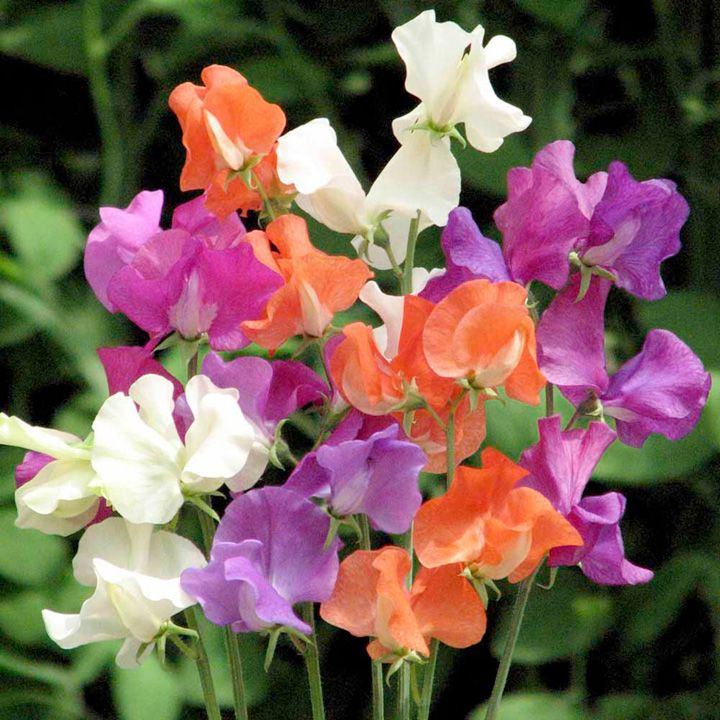
\includegraphics[width=0.96\linewidth]{./images/Pea_lathyrus_odoratus_flower} 

}

\caption{Flower color in lathyrus pea}\label{fig:pea-flower}
\end{figure}

\end{columns}
\end{frame}

\begin{frame}{Quantitative inheritance}
\protect\hypertarget{quantitative-inheritance}{}
\begin{itemize}
\tightlist
\item
  Most of the important variation displayed by nearly all plant traits
  affecting growth, development and reproduction, is quantitative.
\item
  Also called: \emph{Continuous}, \emph{Polygenic variation},
  \emph{Multiple gene controlled traits}
\item
  Demonstrate same basic Mendelian properties for a gene, and also the
  Hardy-Weinberg equilibrium.
\item
  Quantitative characters are governed by several genes; each gene has a
  small effect, which is usually cumulative.
\item
  The environments considerably affect these characters.
\item
  Quantitative characters often show continuous variation with normal
  distribution
\end{itemize}
\end{frame}

\begin{frame}{Qualitative inheritance}
\protect\hypertarget{qualitative-inheritance}{}
\begin{itemize}
\tightlist
\item
  Mendel purposed the law of inheritance based on his studies with
  qualitative characters.
\item
  In the studies of qualitative inheritance, we study phenomena such as:

  \begin{itemize}
  \footnotesize
  \item Dominance, 
  \item Segregation  and independent assortment, 
  \item Gene action and interactions (Epistatis, Masking gene action, Duplicate gene action, Complementary gene action, Additive gene action, Inhibiting gene action, Modifying gene action and Pleiotropy).
  \item Penetrance and expressivity
  \item Linkage
  \end{itemize}
\end{itemize}

\begin{figure}

{\centering 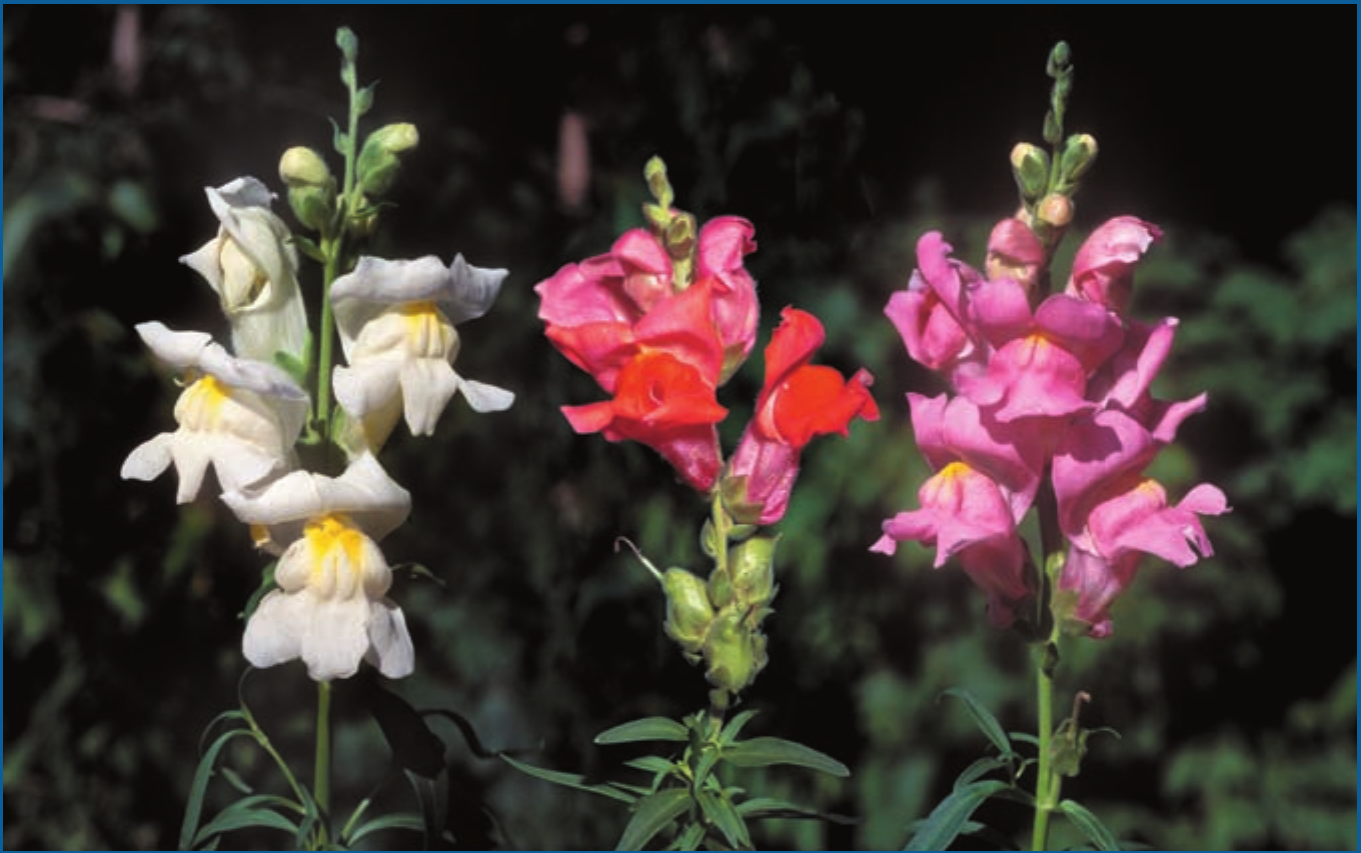
\includegraphics[width=0.38\linewidth]{./images/incomplete_dominance} 

}

\caption{Qualitative inheritance (incomplete dominance); In snapdragons, a heterozygote is pink, intermediate between the two homozygotes red and white. The pink heterozygote demonstrates incomplete dominance.}\label{fig:incomplete-dominance}
\end{figure}
\end{frame}

\begin{frame}{Difference between quantitative and qualitative traits}
\protect\hypertarget{difference-between-quantitative-and-qualitative-traits}{}
\begin{table}

\caption{\label{tab:quant-qual-difference}Difference between qualitative and quantitative traits}
\centering
\fontsize{8}{10}\selectfont
\begin{tabular}[t]{>{\raggedright\arraybackslash}p{18em}>{\raggedright\arraybackslash}p{16em}>{\raggedright\arraybackslash}p{16em}}
\toprule
Character & Qualitative & Quantitative\\
\midrule
\cellcolor{gray!6}{Number of gene and loci controlling the character} & \cellcolor{gray!6}{Few, one (mongenic) or few major genes (oligogenic)} & \cellcolor{gray!6}{Many, polygenes (polygeneic)}\\
Effect of individual gene & Large & Small\\
\cellcolor{gray!6}{Follow mendel's law} & \cellcolor{gray!6}{Yes} & \cellcolor{gray!6}{Yes}\\
Classification on few discrete classes that are easily distinguished & Yes & No\\
\cellcolor{gray!6}{Measurement of the character} & \cellcolor{gray!6}{Observation} & \cellcolor{gray!6}{Measured in metric units}\\
\addlinespace
Frequency distribution & Discrete & Continuous and often normal\\
\cellcolor{gray!6}{Effect of environment on expression of character} & \cellcolor{gray!6}{No or little affected} & \cellcolor{gray!6}{Largely affected}\\
Examples & Disease resistance, Presence of awns, Seed color & Grain yield (kg/ha), Thousand kernel weight (gram)\\
\bottomrule
\end{tabular}
\end{table}
\end{frame}

\begin{frame}{Penetrance}
\protect\hypertarget{penetrance}{}
\footnotesize

\begin{itemize}
\tightlist
\item
  The ability of a gene to express itself in the individuals carrying it
  in the appropriate genotype.
\item
  Generally, oligogenes express themselves in all individuals that carry
  them and their expression is fairly uniform.
\item
  But some oligogenes fail to express themselves in some individuals
  carrying them and are said to have incomplete penetrance.
\item
  Gene expressing itself in every individuals that carries it is said to
  have complete penetrance.
\item
  In the analysis of single-gene inheritance, there is a natural
  tendency to choose mutants that produce clear Mendelian ratios. In
  such cases, we can use the phenotype to distinguish mutant and
  wild-type genotypes with almost 100 percent certainty. In these cases,
  we say that the mutation is 100 percent penetrant into the phenotype.
  However, many mutations show incomplete penetrance: that is, not every
  individual with the genotype expresses the corresponding phenotype.
  Thus, penetrance is defined as the percentage of individuals with a
  given allele who exhibit the phenotype associated with that allele.
\item
  Reasons for incomplete penetrance:

  \begin{itemize}
  \footnotesize
  \item The influence of the environment
  \item The influence of other interacting genes
  \item The subtlety of the mutant phenotype
  \end{itemize}
\end{itemize}
\end{frame}

\begin{frame}{}
\protect\hypertarget{section-2}{}
\begin{figure}

{\centering 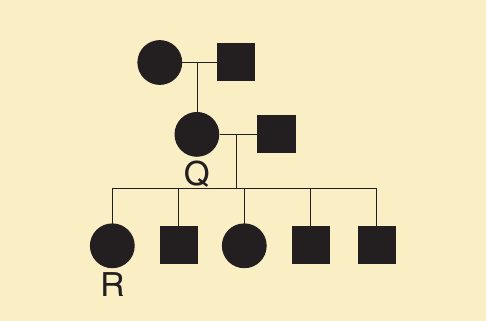
\includegraphics[width=0.6\linewidth]{./images/incomplete_penetrance} 

}

\caption{In this human pedigree of a dominant allele that is not fully penetrant, person Q does not display the phenotype but passed the dominant allele to at least two progeny. Because the allele is not fully penetrant, the other progeny (for example, R) may or may not have inherited the dominant allele.}\label{fig:penetrance}
\end{figure}
\end{frame}

\begin{frame}{Expressivity}
\protect\hypertarget{expressivity}{}
\begin{columns}[T, onlytextwidth]
\column{0.6\textwidth}
\begin{itemize}
\small
\item The ability of a gene to express itself uniformly in all individuals that carry it in the appropriate genotype.
\item A gene that expresses itself uniformly in all individuals has uniform expressivity while those that are unable to do so have variable expressivity. 
\item Expressivity measures the degree to which a given allele is expressed at the phenotypic level; that is, expressivity measures the intensity of the phenotype. For example, "brown" animals (genotype b/b) from different stocks might show very different intensities of brown pigment from light to dark. As for penetrance, variable expressivity may be due to variation in the allelic constitution of the rest of the genome or to environmental factors.
\item Expressivity is indicated as variable or uniform.
\end{itemize}

\column{0.4\textwidth}

\begin{figure}

{\centering 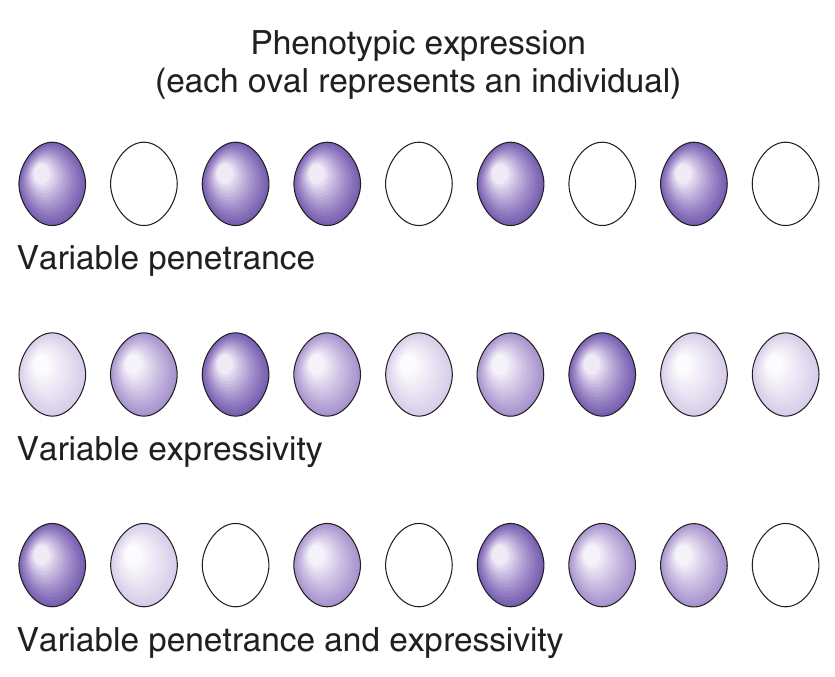
\includegraphics[width=0.9\linewidth]{./images/penetrance_expressivity} 

}

\caption{Assume that all the individuals shown have the same pigment allele (P) and possess the same potential to produce pigment. Effects from the rest of the genome and the environment may suppress or modify pigment production in any one individual. The color indicates the level of expression.}\label{fig:expressivity}
\end{figure}

\end{columns}
\end{frame}

\begin{frame}{Effect in selection}
\protect\hypertarget{effect-in-selection}{}
\begin{itemize}
\tightlist
\item
  Incomplete penetrance and variable expressivity confuse the relation
  between genotype and phenotype.
\item
  Consequently such genes pose difficulty in selection of desired types.
\end{itemize}
\end{frame}

\hypertarget{threshold-characters}{%
\section{Threshold characters}\label{threshold-characters}}

\begin{frame}{Threshold characters}
\begin{itemize}
\tightlist
\item
  Some genes require specific environment, e.g a particular temperature,
  for expression.
\item
  Traits governed by such genes are known as threshold characters.
\item
  For example, a mutant gene in barley produces albino seedlings at
  temperatures below \(8^\circ C\). But when the seedling-carrying gene
  is grown at \(19^\circ C\) or above, they develop into normal green
  seedlings.
\item
  Incomplete penetrance of some genes may be due to a threshold
  requirement.
\end{itemize}
\end{frame}

\hypertarget{multiple-factor-hypothesis}{%
\section{Multiple factor hypothesis}\label{multiple-factor-hypothesis}}

\begin{frame}{}
\protect\hypertarget{section-3}{}
\begin{itemize}
\tightlist
\item
  Many genes with small cumulative effect for any one quantitative
  character account for bell-shaped normal curve appearance of common
  traits. The genetic factors responsible for this type of effects were
  termed as multiple factors.
\item
  Now multiple factor has been replaced by polygene or multiple genes
  (purposed by Mather).
\item
  In 1908, Nilsson-Ehle presented experiment evidence to support this
  hypothesis by studying seed color in wheat and oats (demonstrated an
  actual segregation and assortment of genes with quantitative effect).
\item
  Nilsson-Ehle crossed two varieties of wheat, one with deep red grain
  of genotype \(R_1R_1R_2R_2\), and the other white grain of genotype
  \(r_1r_1r_2r_2\).
\item
  The distribution of resulting individuals from cross was explained on
  the basis of two pairs of genes segregating independently, which each
  dominant allele adding to the intensity of the red color.
\item
  Two or more non allelic genes that affect in similar way of
  development of a quantitative character are called multiple genes or
  polygenes.
\end{itemize}
\end{frame}

\begin{frame}{Multiple factor hypothesis (Example)}
\protect\hypertarget{multiple-factor-hypothesis-example}{}
\begin{itemize}
\tightlist
\item
  According to Nilsson-ehle, there were three individual gene pairs
  involved in determination of grain color in wheat, i.e., Aa, Bb, Cc,
  with genes for red (ABC) dominant over genes for white (abc). Each of
  these three gene pairs segregated in predictable mendelian fashion, so
  that the products of heterozygotes for any one pair, i.e.~Aa x Ax,
  produced offspring in the ratio 3 red (A\_):1 white (aa). When two
  gene-pair differences were segregating at the same time in
  Nilsson-Ehle's experiments, i.e., AaBb x AaBb, the results also
  followed mendelian principles, producing a ratio 15 red (A\_B\_,
  A\_bb, aaB\_): 1 white (aabb). Similarly a cross between heterozygotes
  for three gene paris produced a close fit to the predicted ratio 63
  red: 1 white
  \footnote[frame]{Refer to Chapter 14: Quantitative inheritance, Genetics, Monroe. M. Strickberger, Page 245}.
\end{itemize}
\end{frame}

\begin{frame}{}
\protect\hypertarget{section-4}{}
\begin{table}

\caption{\label{tab:wheat-experiment}Wheat seed color variation; An example case of multiple factor trait expression}
\centering
\fontsize{8}{10}\selectfont
\begin{tabular}[t]{>{\raggedleft\arraybackslash}p{6em}>{\raggedleft\arraybackslash}p{7em}>{\raggedleft\arraybackslash}p{7em}>{\raggedleft\arraybackslash}p{6em}>{\raggedleft\arraybackslash}p{6em}}
\toprule
Number of genotypes & F2 genotypes & Color & Number of plants (Phenotype) & Number of dominant genes\\
\midrule
\cellcolor{gray!6}{1} & \cellcolor{gray!6}{R1R1R2R2} & \cellcolor{gray!6}{Very dark red} & \cellcolor{gray!6}{1} & \cellcolor{gray!6}{4}\\
2 & R1R1R2r2 & Dark red & 4 & 3\\
\cellcolor{gray!6}{2} & \cellcolor{gray!6}{R1r2R2R2} & \cellcolor{gray!6}{Dark red} & \cellcolor{gray!6}{} & \cellcolor{gray!6}{3}\\
1 & R1R1r2r2 & Medium red & 6 & 2\\
\cellcolor{gray!6}{4} & \cellcolor{gray!6}{R1r1R2r2} & \cellcolor{gray!6}{Medium red} & \cellcolor{gray!6}{} & \cellcolor{gray!6}{2}\\
\addlinespace
1 & R1R1R2R2 & Medium red &  & 2\\
\cellcolor{gray!6}{2} & \cellcolor{gray!6}{R1r1r2r2} & \cellcolor{gray!6}{Light red} & \cellcolor{gray!6}{4} & \cellcolor{gray!6}{1}\\
2 & r1r1R2r2 & Light red &  & 1\\
\cellcolor{gray!6}{1} & \cellcolor{gray!6}{r1r1r2r2} & \cellcolor{gray!6}{White} & \cellcolor{gray!6}{1} & \cellcolor{gray!6}{0}\\
\bottomrule
\end{tabular}
\end{table}
\end{frame}

\hypertarget{transgressive-segregation}{%
\section{Transgressive segregation}\label{transgressive-segregation}}

\begin{frame}{}
\protect\hypertarget{section-5}{}
\begin{itemize}
\tightlist
\item
  Appearance of features that are unlike either parent.
\item
  Quantitative character of progeny may fall outside the range of
  parents is called transgressive segregation.
\item
  Transgressive segregation is used extensively by breeders to obtain
  segregates following a cross that are superior to the parental strains
  for traits inherited in a quantitative manner.
\end{itemize}

\begin{center}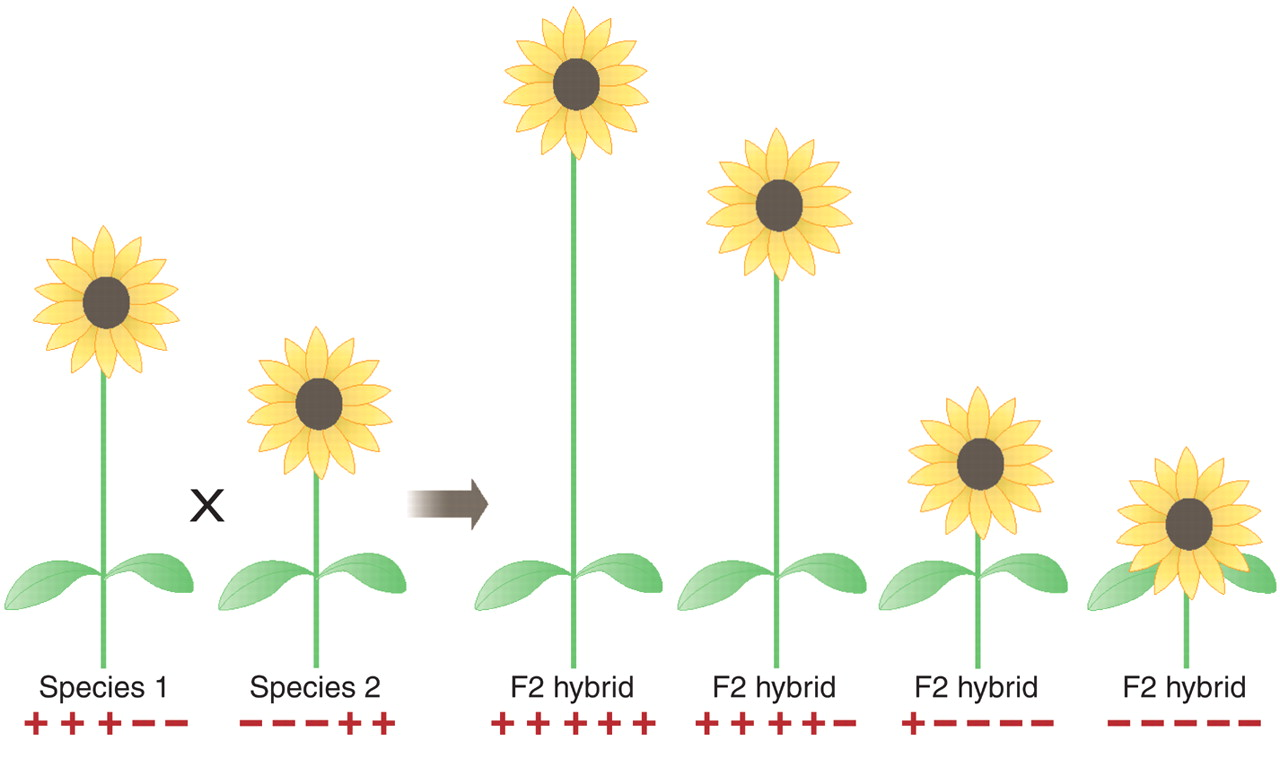
\includegraphics[width=0.5\linewidth]{./images/transgressive_segregation} \end{center}
\end{frame}

\begin{frame}{Multigenic and multiallelic inheritance}
\protect\hypertarget{multigenic-and-multiallelic-inheritance}{}
\begin{columns}[T, onlytextwidth]

\column{0.6\textwidth}

\begin{block}{Multiallelic inheritance}

For given number of alleles in a locus, number of genotype combinations possible is shown on the graph \ref{fig:polymorphic-alleles-locus}.
\end{block}

\begin{figure}

{\centering \includegraphics[width=0.85\linewidth]{04-qualitative_and_quantitative_characters_pdf_files/figure-beamer/polymorphic-alleles-locus-1} 

}

\caption{Exponential increase in the number of genotypes with increasing level of polymorphism for a given diploid locus.}\label{fig:polymorphic-alleles-locus}
\end{figure}

\hspace{-0.4cm}\column{0.36\textwidth}
\begin{block}{Multigenic inheritance}
\small
For given number of biallelic loci, number of genotype combinations possible in $F_2$ after random mating are:

$$
\small
\text{Numer of genotypes} = 3^n
$$
Where, $n$ is the total number of biallelic loci. 
\end{block}
\end{columns}
\end{frame}

\begin{frame}{Numerical problem}
\protect\hypertarget{numerical-problem}{}
The leaves of pineapples can be classified into three types: spiny (S),
spiny tip (ST), and piping (nonspiny; P). In crosses between pure
strains followed by intercrosses of the F1, the following results
appeared:

\begin{center}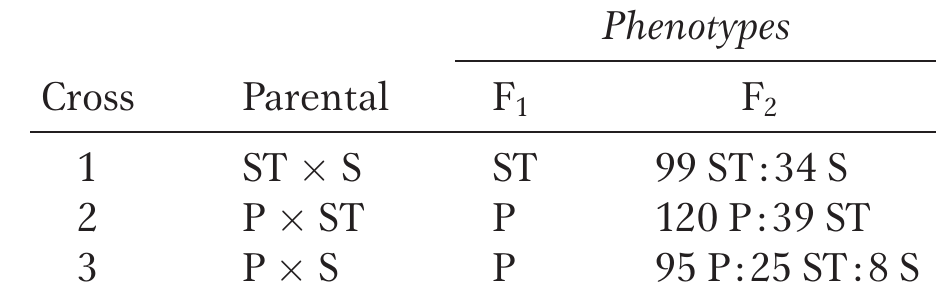
\includegraphics[width=0.4\linewidth]{./images/pineapple_genetics} \end{center}

\begin{enumerate}
[a.]
\tightlist
\item
  Assign gene symbols. Explain these results in regard to the genotypes
  produced and their ratios.
\item
  Using the model from part a, give the phenotypic ratios that you would
  expect if you crossed (1) the F1 progeny from piping ? spiny with the
  spiny parental stock and (2) the F1 progeny of piping ? spiny with the
  F1 progeny of spiny ? spiny tip.
\end{enumerate}
\end{frame}

\begin{frame}{Solution 1}
\protect\hypertarget{solution-1}{}
\footnotesize

First, let's look at the F2 ratios. We have clear 3 : 1 ratios in
crosses 1 and 2, indicating single-gene segregations. Cross 3, however,
shows a ratio that is almost certainly a 12 : 3 : 1 ratio. How do we
know this ratio? Well, there are simply not that many complex ratios in
genetics, and trial and error brings us to the 12 : 3 : 1 quite quickly.
In the 128 progeny total, the numbers of 96 : 24 : 8 are expected, but
the actual numbers fit these expectations remarkably well.

One of the principles of this chapter is that modified Mendelian ratios
reveal gene interactions. Cross 3 gives F2 numbers appropriate for a
modified dihybrid Mendelian ratio, and so it looks as if we are dealing
with a two-gene interaction. It seems the most promising place to start;
we can return to crosses 1 and 2 and try to fit them in later.

Any dihybrid ratio is based on the phenotypic proportions 9 : 3 : 3 : 1.
Our observed modification groups them as follows:

\[
\small
\begin{aligned}
9A/\_;B/\_ &~& 9~piping \\
3A/\_;b/b &~& 3~piping \\
3a/a;B/\_ &~& 3~spiny~tip \\
1a/a;b/b &~& 1~spiny
\end{aligned}
\]
\end{frame}

\begin{frame}{}
\protect\hypertarget{section-6}{}
So, without worrying about the name of the type of gene interaction (we
are not asked to supply this anyway), we can already define our three
pineapple-leaf phenotypes in relation to the proposed allelic pairs A/a
and B/b:

\[
\small
\begin{aligned}
piping &=& A/\_ (B/b~irrelevant) \\
spiny tip &=& a/a; B/\_ \\
spiny &=& a/a; b/b
\end{aligned}
\]

What about the parents of cross 3 ? The spiny parent must be a/a ; b/b,
and, because the B gene is needed to produce F2 spiny-tip leaves, the
piping parent must be A/A ; B/B. (Note that we are told that all parents
are pure, or homozygous.) The F1 must therefore be A/a ; B/b. Without
further thought, we can write out cross 1 as follows:
\end{frame}

\begin{frame}{}
\protect\hypertarget{section-7}{}
\footnotesize

\begin{center}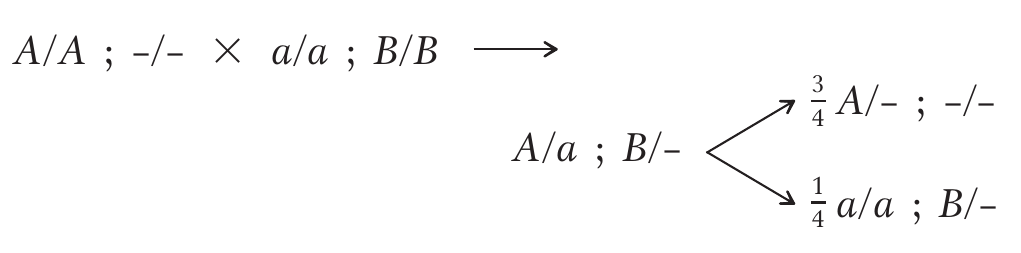
\includegraphics[width=0.34\linewidth]{./images/cross2_ab} \end{center}

\begin{center}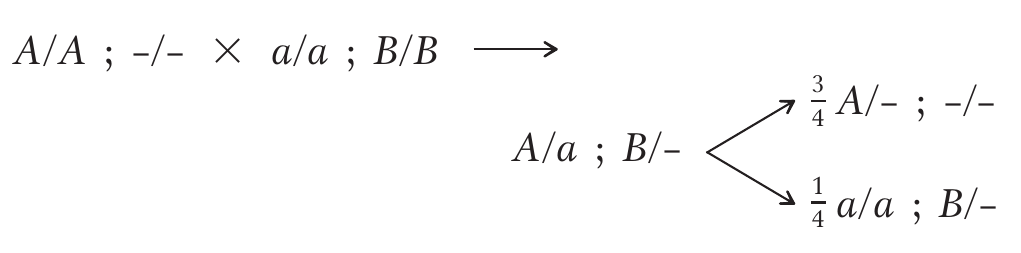
\includegraphics[width=0.34\linewidth]{./images/cross2_ab} \end{center}

We know that the F2 of cross 2 shows single-gene segregation, and it
seems certain now that the A/a allelic pair has a role. But the B allele
is needed to produce the spiny-tip phenotype, and so all plants must be
homozygous B/B:

\begin{center}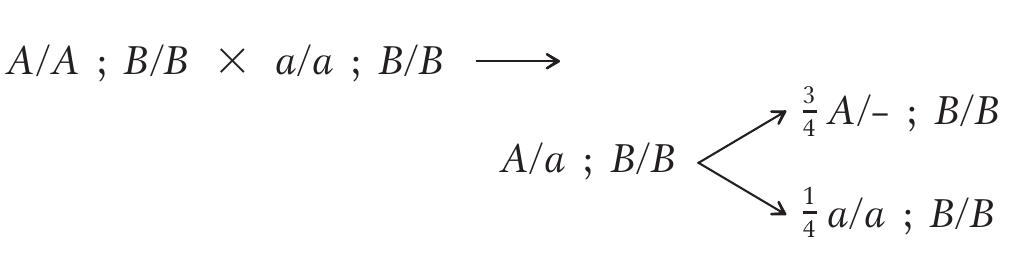
\includegraphics[width=0.34\linewidth]{./images/cross_multiple} \end{center}

Notice that the two single-gene segregations in crosses 1 and 2 do not
show that the genes are not interacting. What is shown is that the
two-gene interaction is not revealed by these crosses-only by cross 3,
in which the F1 is heterozygous for both genes.
\end{frame}

\begin{frame}{}
\protect\hypertarget{section-8}{}
\begin{enumerate}
[a.]
\setcounter{enumi}{1}
\tightlist
\item
  Now it is simply a matter of using Mendel's laws to predict cross
  outcomes:
\end{enumerate}

\begin{center}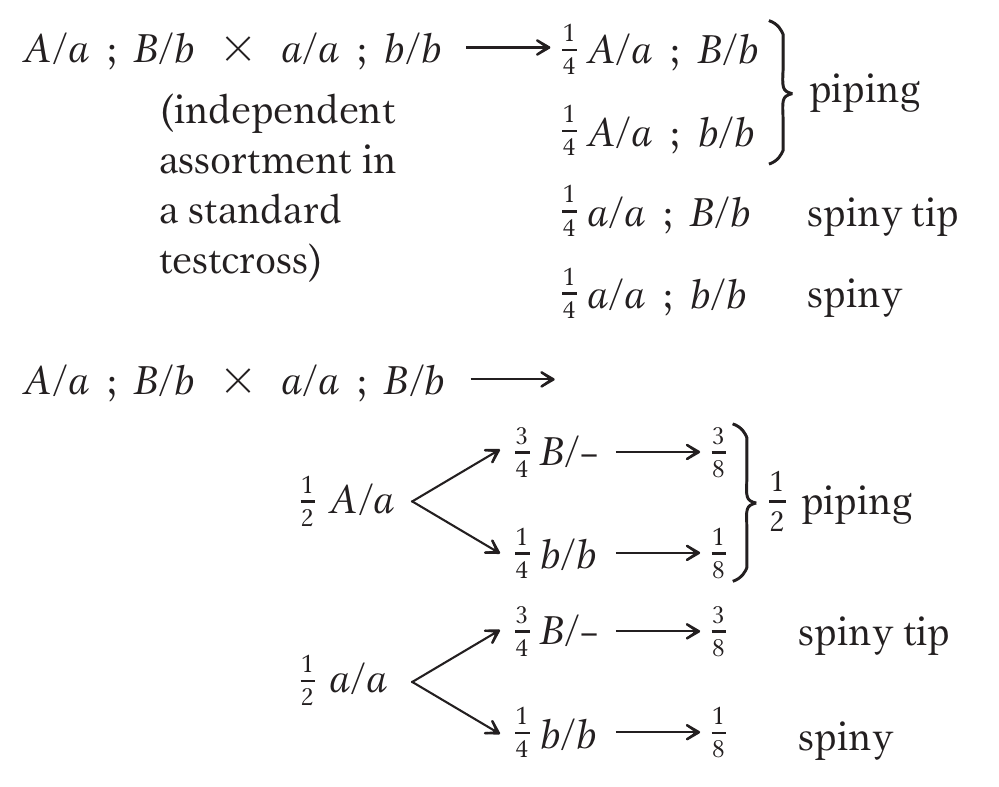
\includegraphics[width=0.4\linewidth]{./images/trait_genetics} \end{center}
\end{frame}

\hypertarget{gene-action-and-interaction}{%
\section{Gene action and
interaction}\label{gene-action-and-interaction}}

\begin{frame}{}
\protect\hypertarget{section-9}{}
\begin{columns}[T,onlytextwidth,c]

\column{0.7\textwidth}

\begin{table}

\caption{\label{tab:gene-action-interaction-types}Types of gene action and interaction. (Adapted from Comstock (1964)).}
\centering
\fontsize{6}{8}\selectfont
\begin{tabular}[t]{llrrr}
\toprule
 & Genotypes & AA & Aa & aa\\
\midrule
\addlinespace[0.3em]
\multicolumn{5}{l}{\textbf{Additive genes effects}}\\
\hspace{1em} & BB & 4 & 3 & 2\\
\cmidrule{2-5}
\hspace{1em} & Bb & 3 & 2 & 1\\
\cmidrule{2-5}
\hspace{1em} & bb & 2 & 1 & 0\\
\cmidrule{1-5}
\addlinespace[0.3em]
\multicolumn{5}{l}{\textbf{Dominance gene effects}}\\
\hspace{1em} & BB & 4 & 4 & 2\\
\cmidrule{2-5}
\hspace{1em} & Bb & 4 & 4 & 2\\
\cmidrule{2-5}
\hspace{1em} & bb & 2 & 2 & 0\\
\cmidrule{1-5}
\addlinespace[0.3em]
\multicolumn{5}{l}{\textbf{Epistatic genes effects}}\\
\hspace{1em} & BB & 4 & 4 & 0\\
\cmidrule{2-5}
\hspace{1em} & Bb & 4 & 4 & 0\\
\cmidrule{2-5}
\hspace{1em} & bb & 0 & 0 & 0\\
\cmidrule{1-5}
\addlinespace[0.3em]
\multicolumn{5}{l}{\textbf{Overdominance gene effect}}\\
\hspace{1em} & BB & 2 & 3 & 1\\
\cmidrule{2-5}
\hspace{1em} & Bb & 3 & 4 & 2\\
\cmidrule{2-5}
\hspace{1em} & bb & 1 & 2 & 0\\
\bottomrule
\end{tabular}
\end{table}

\column{0.3\textwidth}

\footnotesize Refer to Lecture slides of Introductory Genetics on "Gene Action and Interaction".

\end{columns}
\end{frame}

\hypertarget{continuous-variation}{%
\section{Continuous variation}\label{continuous-variation}}

\begin{frame}{Number of genes contributing to a quantitative character}
\protect\hypertarget{number-of-genes-contributing-to-a-quantitative-character}{}
A formula has been purposed for estimating the number of genes n
involved in the inheritance of a quantitative character.

\[n = \frac{(\bar{P_1} -\bar{P_2})^2}{8[\sigma_{F_2}^2-\sigma_{F_1}^2]}\]

Where, \(\bar{P_1}\) and \(\bar{P_2}\) are trait means of inbred parents
\(P_1\) and \(P_2\), respectively. \(\sigma_{F_2}^2\) and
\(\sigma_{F_1}^2\) are standard deviation of \(F_2\) and \(F_1\),
respectively.
\end{frame}

\begin{frame}{Components of variation of a quantitative character}
\protect\hypertarget{components-of-variation-of-a-quantitative-character}{}
\footnotesize

\begin{itemize}
\tightlist
\item
  Quantitative characters are more affected by environments.
\item
  Phenotypic performance of genotypes evaluated in varied environmental
  conditions (MET) may be described according to a mathematical model to
  facilitate statistical analysis and interpretation.
\item
  Yield (and quantitative characters alike) data show Genotype by
  Environment (G x E) interaction -- genotypes respond differently to
  different
  environments\footnote[frame]{For a detailed discussion of G x E and interpretation, refer to lecture slide on G x E from Molecular and Population Genetics course}.
\item
  A traditional approach to the analysis of G x E is a two-way analysis
  of variance (ANOVA) model where genotype, environment, and their
  interaction are treated as fixed effects with the model:
\end{itemize}

\[
y_{ijk} = \mu + g_{i} + e_{j} + ge_{ij} + \epsilon_{ijk}
\]

where, \(y_{ijk}\) is the yield of the \(k^{\text{th}}\) replicate of
the \(i^{\text{th}}\) genotype in the \(j^{\text{th}}\) environment,
\(\mu\) is the overall mean (mean of all the possible genotypes grown
under all possible environments), \(g_{i}\) = is the fixed effect of the
\(i^{\text{th}}\) genotype, \(e_{j}\) is the fixed effect of the
\(j^{\text{th}}\) environment, \(ge_{ij}\) is the interaction between
\(i^{\text{th}}\) genotype and the \(j^{\text{th}}\) environment, and
\(\epsilon_{ijk}\) is the experimental error associated with the
\(ijk^{\text{th}}\) observation.
\end{frame}

\begin{frame}{Paritioning of variance components}
\protect\hypertarget{paritioning-of-variance-components}{}
\begin{table}

\caption{\label{tab:anova-var-partitioning}Analysis of variance (and broad sense heritability estimates in the case of a series of g genotypes evaluated across e environments)}
\centering
\fontsize{8}{10}\selectfont
\begin{tabular}[t]{>{\raggedright\arraybackslash}p{12em}>{\raggedright\arraybackslash}p{5em}>{\raggedright\arraybackslash}p{7em}>{\raggedright\arraybackslash}p{12em}}
\toprule
Source of variation & Degrees of freedom & Mean squares & Expected mean squares\\
\midrule
\cellcolor{gray!6}{Environment} & \cellcolor{gray!6}{e-1} & \cellcolor{gray!6}{} & \cellcolor{gray!6}{$\sigma^2 + g \sigma^2_{r(E)} + r \sigma^2_{GE} + rg \sigma^2_{E}$}\\
Rep (Environment) & (r-1)e &  & $\sigma^2_{e} + g \sigma^2_{r(E)}$\\
\cellcolor{gray!6}{Genotype} & \cellcolor{gray!6}{g-1} & \cellcolor{gray!6}{$MS_G$} & \cellcolor{gray!6}{$\sigma^2_e + r \sigma^2_{GE} + re \sigma^2_{G}$}\\
Genotype x Environment & (g-1)(e-1) & $MS_{GE}$ & $\sigma^2_{e} + r \sigma^2_{GE}$\\
\cellcolor{gray!6}{Error} & \cellcolor{gray!6}{(g-1)(r-1)e} & \cellcolor{gray!6}{$MS_{E}$} & \cellcolor{gray!6}{$\sigma^2_{e}$}\\
\bottomrule
\end{tabular}
\end{table}

Total phenotypic variance
(\(Var(Y_{ijk}) = \hat{\sigma}^2_{P} = \hat{\sigma}^2_{e} + \hat{\sigma}^2_{GE} + \hat{\sigma}^2_{G}\))

Phenotypic variance of genotypic means
(\(Var(\bar{Y}_{ijk}) = \hat{\sigma}^2_{\bar{P}} = \frac{\hat{\sigma}^2_{e}}{re} + \frac{\hat{\sigma}^2_{GE}}{e} + \hat{\sigma}^2_{G}\)
= \(\frac{MS_G}{re}\))

Genotypic variance = \(\hat{\sigma}^2_{G} = \frac{MS_G - MS_{GE}}{re}\)
\end{frame}

\hypertarget{heritability}{%
\section{Heritability}\label{heritability}}

\begin{frame}{Meaning}
\protect\hypertarget{meaning}{}
\small

\begin{itemize}
\tightlist
\item
  To make economically meaningful progress in an organized programme of
  selective breeding, two conditions must be met;

  \begin{itemize}
  \footnotesize
  \item There must be some observable phenotypic variation within the crop. This would normally be expected, even if it were due entirely to the effects of a variable environment.
  \item At least some of this phenotypic variation must have a genetic basis.
  \end{itemize}
\item
  This leads to the concept of heritability (\(h^2\)), which is the
  proportion of phenotypic variance that is genetic in origin.
\item
  The values of \(h^2\) can range from 0 to 1. If \(h^2\) is close to
  zero, there will be little scope for advancement and there would be
  little point in trying to improve this character in a plant breeding
  program.
\item
  There are three main ways of estimating heritability:

  \begin{itemize}
  \footnotesize
  \item Carrying out particular genetic crosses and observing the performance of their progeny so that the resulting data can be partitioned into genetic and environmental components.
  \item Based on the direct measurement of the degree of resemblance between offspring and one, or both, of their parents. This is achieved by regression of the former onto the latter in the absence of selection.
  \item Measuring the response of a population to given levels of selection.
  \end{itemize}
\end{itemize}
\end{frame}

\begin{frame}{}
\protect\hypertarget{section-10}{}
\begin{block}{Broad sense heritability}
\protect\hypertarget{broad-sense-heritability}{}
\footnotesize

\begin{itemize}
\tightlist
\item
  The total genetic varinace divided by the total phenotypic variance is
  Broad-sense heritability (\(h_b^2\)).
\item
  This estimation uses the total genetic variance in a
  additive-dominance model, while the total phenotypic variance is
  obtained by adding environmental variance to this genetic variance.
\end{itemize}

\[
\small
h_b^2 = \frac{V_A + V_D}{V_A + V_D + V_E}
\]

\begin{itemize}
\tightlist
\item
  Dominant genetic variance will be dependent upon the degree of
  heterozygosity in the population and will differ between fillial
  generations.
\end{itemize}
\end{block}

\begin{block}{Narrow sense heritability}
\protect\hypertarget{narrow-sense-heritability}{}
\footnotesize

\begin{itemize}
\tightlist
\item
  A more useful form of heritability for plant breeders, therefore, is
  \emph{narrow-sense heritability} (\(h_n^2\)), which is:
\end{itemize}

\[
\small
h_n^2 = \frac{V_A}{V_A+V_D+V_E}
\]

\begin{itemize}
\tightlist
\item
  In estimation of \(h^2_n\) genetic relationships among relatives
  (lineal (parent-offspring) or collateral (full-or half-sibs)) are
  used.
\end{itemize}
\end{block}
\end{frame}

\begin{frame}{Calculation}
\protect\hypertarget{calculation}{}
\small

\begin{itemize}
\tightlist
\item
  Variance based approaches (Useful for both broad and narrow sense
  heritability estimation) - ratio of variance
  estimates\footnote[frame]{Refer to previous section on partitioning of variance.}

  \begin{itemize}
  \tightlist
  \item
    Variance based approach still has two basis for obtaining
    heritability estimates -- individual experimental unit basis
    (Equation (i)) and genotypic-mean basis (Equation (ii)).
  \end{itemize}
\end{itemize}

\[
\small
\begin{aligned}
h_{bs}^2 &= \frac{\sigma^2_{G}}{\sigma^2_{P}} \\
h_{ns}^2 &= \frac{\sigma^2_{A}}{\sigma^2_{P}}
\end{aligned}
\]

\[
\small
h^2_{bi} = \frac{\hat{\sigma}^2_G}{\hat{\sigma}^2_G + \hat{\sigma}^2_{GE} + \hat{\sigma}^2_e}
\tag{i}
\]

\[
\small
h^2_{bm} = \frac{\hat{\sigma}^2_G}{\hat{\sigma}^2_G + \frac{\hat{\sigma}^2_{GE}}{e} + \frac{\hat{\sigma}^2_e}{re}}
\tag{ii}
\]
\end{frame}

\begin{frame}{}
\protect\hypertarget{section-11}{}
\begin{itemize}
\tightlist
\item
  Realized heritability

  \begin{itemize}
  \tightlist
  \item
    Heritability estimated using the amount of genetic gain that is
    realized by selection within a population (Falconer and Mackay,
    1996).
  \end{itemize}
\end{itemize}

\[
\small
h^2 = \frac{R}{S}
\]

\begin{itemize}
\tightlist
\item
  Six generation mean analysis method

  \begin{itemize}
  \tightlist
  \item
    Phenotypic mean values of each (P1, P2, F1, BCP1, BCP2, and F2)
    generation is required.
  \end{itemize}
\end{itemize}
\end{frame}

\begin{frame}{}
\protect\hypertarget{section-12}{}
\begin{itemize}
\tightlist
\item
  Parent offspring regression

  \begin{itemize}
  \tightlist
  \item
    This method is based on how much does the resemblance parents and
    offspring exist.
  \item
    If there is perfect resemblance between parents and offspring, then,
    \(b = 1\) and there is perfect heritable genetic effect.
  \item
    On contrary if there is no resemblance between parents and offspring
    \(b = 0\), and there is no heritable effect but variation is only
    due to environment.
  \item
    Therefore, narrow sense heritability (
    \(b = h_{ns}^2 = \frac{VA}{VP}\) )
  \item
    If only one parent is known (animal experiments or polycrosses):
  \end{itemize}
\end{itemize}

\[
\small
\begin{aligned}
b &= \frac{1}{2}.\frac{Va}{VP}\\
h_{ns}^2 &= 2b
\end{aligned}
\]

where, \(b\) = slope of parent offspring regression line
\end{frame}

\begin{frame}{}
\protect\hypertarget{section-13}{}
\begin{table}

\caption{\label{tab:heritability-estimates}Heritability estimates of some common plant architectural traits; Source: Acquaah, 2014}
\centering
\begin{tabular}[t]{lr}
\toprule
Trait & Heritability\\
\midrule
\cellcolor{gray!6}{Plant height} & \cellcolor{gray!6}{45}\\
Hypocotyl diameter & 38\\
\cellcolor{gray!6}{Number of branches/plant} & \cellcolor{gray!6}{56}\\
Nodes in lower third & 36\\
\cellcolor{gray!6}{Nodes in mid section} & \cellcolor{gray!6}{45}\\
\addlinespace
Nodes in upper third & 46\\
\cellcolor{gray!6}{Pods in lower third} & \cellcolor{gray!6}{62}\\
Pods in mid section & 85\\
\cellcolor{gray!6}{Pods in upper third} & \cellcolor{gray!6}{80}\\
Pod width & 81\\
\addlinespace
\cellcolor{gray!6}{Pod length} & \cellcolor{gray!6}{67}\\
Seed number per pod & 30\\
\cellcolor{gray!6}{100 seed weight} & \cellcolor{gray!6}{77}\\
\bottomrule
\end{tabular}
\end{table}
\end{frame}

\hypertarget{numerical-problem-1}{%
\section{Numerical problem}\label{numerical-problem-1}}

\begin{frame}{}
\protect\hypertarget{section-14}{}
\begin{enumerate}
\item
  Two pure lines of rice are crossed. In the \(F_1\) the variance in
  spike length is 1.5. The F1 is selfed. In the \(F_2\) the variance in
  spike length is 4.5. Estimate broad sense heritability of spike length
  in rice
\item
  The phenotypic variance of yield in maize 200 \(kg^2\) per acre. The
  variance within an inbred line is 80. The regression of offspring
  phenotype on mid parent values is 0.32. Find additive variance,
  genetic variance, environmental variance, narrow sense heritability
  and broad sense heritability.
\end{enumerate}
\end{frame}

\begin{frame}{}
\protect\hypertarget{section-15}{}
\begin{enumerate}
\setcounter{enumi}{2}
\tightlist
\item
  Estimate heritability through parent offspring regression method from
  the following available data.
\end{enumerate}

\begin{table}
\centering
\begin{tabular}{rr}
\toprule
Mid parent value (X) & Individual offspring (Y)\\
\midrule
\cellcolor{gray!6}{20} & \cellcolor{gray!6}{25}\\
18 & 21\\
\cellcolor{gray!6}{15} & \cellcolor{gray!6}{20}\\
17 & 20\\
\cellcolor{gray!6}{21} & \cellcolor{gray!6}{26}\\
\addlinespace
22 & 25\\
\bottomrule
\end{tabular}
\end{table}
\end{frame}

\begin{frame}{}
\protect\hypertarget{section-16}{}
\begin{enumerate}
\setcounter{enumi}{3}
\tightlist
\item
  Suppose 2 inbred lines A and B are crossed to produce hybrid. The
  genotype of A is AAbbccDDEEFF and the genotype of B is aaBBCCddeeFF.
  A, B, C, D, E and F are the dominant genes. If dominant homozygote
  contributes 2 \(ton~ha^{-1}\), recessive homozygote contributes 1
  \(ton~ha^{-1}\) and heterozygote contributes 2.5 \(ton~ha^{-1}\), Find
  the grain yields of Parent A, Parent B and \(F_1\) hybrid on the basis
  of dominance and over-dominance hypothesis.
\end{enumerate}
\end{frame}




\end{document}
